\documentclass[11pt,a4paper]{article}

% ------------------------------------------------------------
% Paquetes
% ------------------------------------------------------------
\usepackage[utf8]{inputenc}
\usepackage[T1]{fontenc}
\usepackage[spanish,es-nodecimaldot]{babel}
\usepackage[a4paper,margin=2.2cm]{geometry}
\usepackage[table]{xcolor}
\usepackage{graphicx}
\usepackage{booktabs}
\usepackage{tabularx}
\usepackage{array}
\usepackage{enumitem}
\usepackage{listings}
\usepackage[most]{tcolorbox}
\usepackage{fancyhdr}
\usepackage{titlesec}
\usepackage{hyperref}
\usepackage{microtype}

% ------------------------------------------------------------
% Identidad visual
% ------------------------------------------------------------
\definecolor{zombieDark}{HTML}{111820}
\definecolor{zombieGreen}{HTML}{87A96B}
\definecolor{zombieLight}{HTML}{EEF3E8}
\definecolor{warningOrange}{HTML}{D9822B}
\definecolor{metalBlue}{HTML}{40576D}
\definecolor{softGray}{HTML}{F3F5F7}
\definecolor{textDark}{HTML}{20262D}

\hypersetup{
  colorlinks=true,
  linkcolor=metalBlue,
  urlcolor=warningOrange,
  pdftitle={Documentación de ZombieTech},
  pdfauthor={Romario Anchaise}
}

\titleformat{\section}
  {\Large\bfseries\color{zombieDark}}
  {\thesection}{0.7em}{}
\titleformat{\subsection}
  {\large\bfseries\color{metalBlue}}
  {\thesubsection}{0.7em}{}

\pagestyle{fancy}
\fancyhf{}
\fancyhead[L]{\textbf{ZombieTech}}
\fancyhead[R]{Documentación del proyecto}
\fancyfoot[C]{\thepage}
\renewcommand{\headrulewidth}{0.4pt}

\setlist[itemize]{leftmargin=1.5em,itemsep=0.25em}
\setlist[enumerate]{leftmargin=1.7em,itemsep=0.3em}
\renewcommand{\arraystretch}{1.25}

\newtcolorbox{gamebox}[1]{
  enhanced,
  breakable,
  colback=zombieLight,
  colframe=zombieGreen,
  boxrule=0.8pt,
  arc=2mm,
  title=\textbf{#1},
  coltitle=white,
  colbacktitle=zombieGreen
}

\newtcolorbox{unitybox}[1]{
  enhanced,
  breakable,
  colback=softGray,
  colframe=metalBlue,
  boxrule=0.8pt,
  arc=2mm,
  title=\textbf{Dónde está en Unity: #1},
  coltitle=white,
  colbacktitle=metalBlue
}

\newtcolorbox{warningbox}[1]{
  enhanced,
  breakable,
  colback=warningOrange!8,
  colframe=warningOrange,
  boxrule=0.8pt,
  arc=2mm,
  title=\textbf{#1},
  coltitle=white,
  colbacktitle=warningOrange
}

\lstdefinestyle{projecttree}{
  basicstyle=\ttfamily\small,
  backgroundcolor=\color{zombieDark},
  basicstyle=\ttfamily\small\color{white},
  frame=single,
  rulecolor=\color{metalBlue},
  breaklines=true,
  columns=fullflexible,
  showstringspaces=false
}

\lstdefinestyle{codestyle}{
  language=[Sharp]C,
  basicstyle=\ttfamily\footnotesize,
  keywordstyle=\color{metalBlue}\bfseries,
  stringstyle=\color{warningOrange},
  commentstyle=\color{zombieGreen!70!black},
  backgroundcolor=\color{softGray},
  frame=single,
  rulecolor=\color{metalBlue!50},
  breaklines=true,
  columns=fullflexible,
  showstringspaces=false,
  tabsize=2
}

\newcommand{\component}[1]{\textbf{\textcolor{metalBlue}{#1}}}
\newcommand{\keycap}[1]{\fcolorbox{metalBlue}{softGray}{\texttt{#1}}}

\begin{document}

% ------------------------------------------------------------
% Portada
% ------------------------------------------------------------
\begin{titlepage}
  \pagecolor{zombieDark}
  \color{white}
  \centering
  \vspace*{1.2cm}

  {\Huge\bfseries ZOMBIETECH\par}
  \vspace{0.25cm}
  {\Large Videojuego 2D de plataformas y supervivencia\par}
  \vspace{0.9cm}

  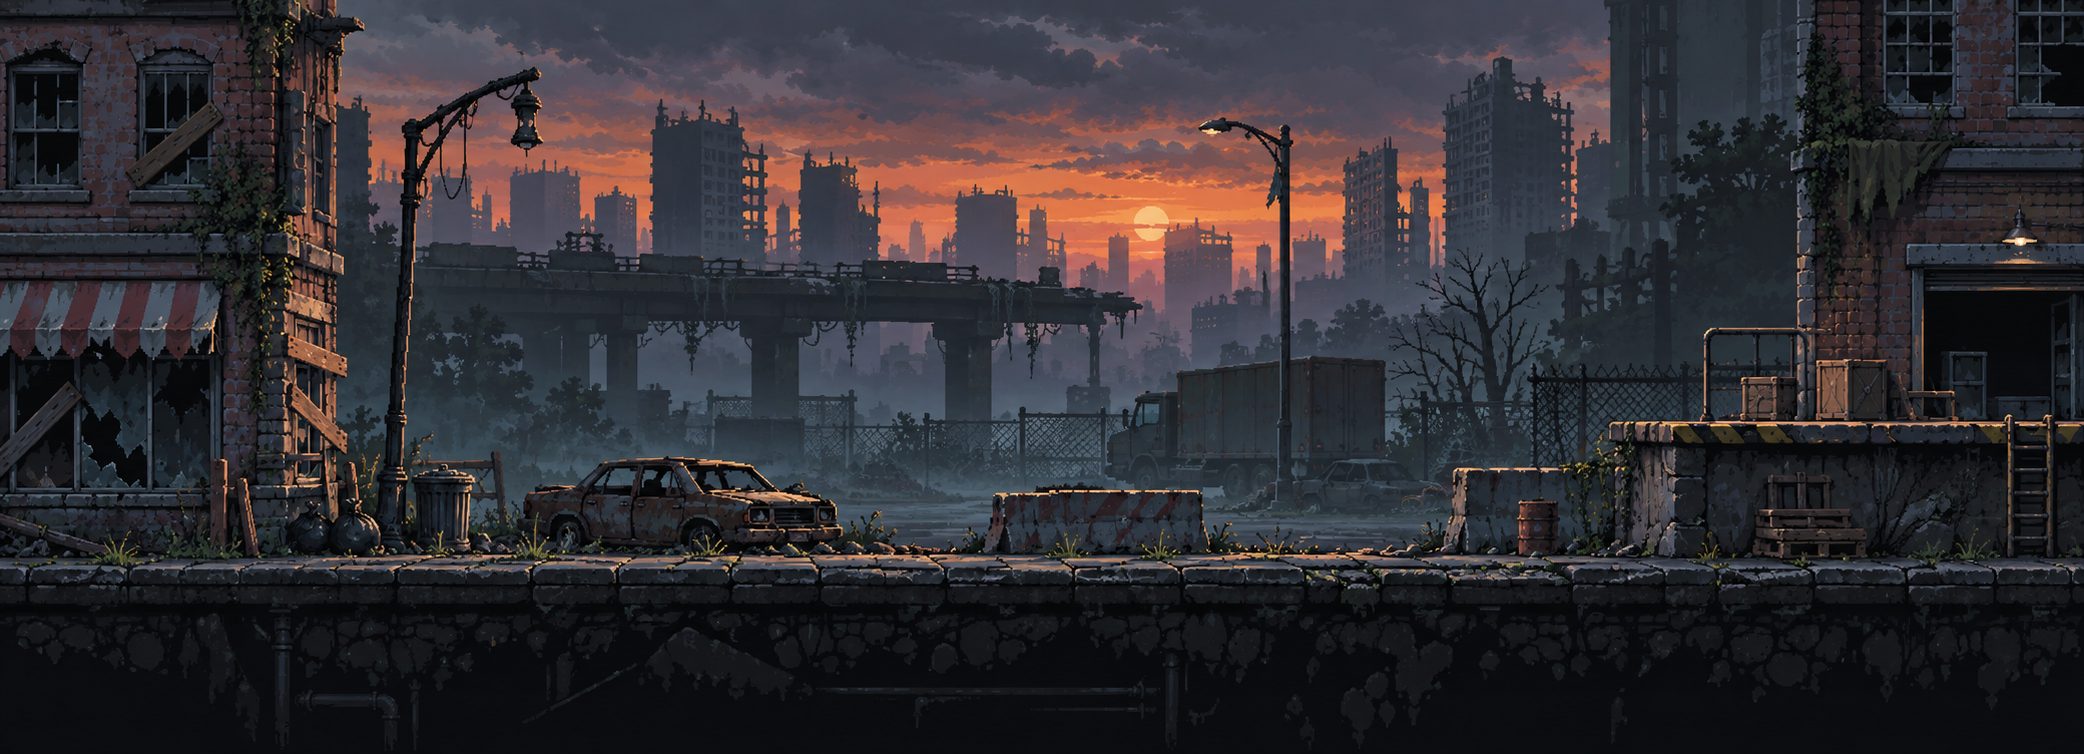
\includegraphics[width=\textwidth,height=0.43\textheight,keepaspectratio]{Assets/Art/Backgrounds/ZombieCityBackground.png}

  \vfill
  \begin{tcolorbox}[colback=white!8,colframe=zombieGreen,width=0.78\textwidth,arc=3mm]
    \centering\color{white}
    \textbf{Autor:} Romario Anchaise\\[0.2cm]
    \textbf{Motor:} Unity 6.3 LTS\\[0.2cm]
    \textbf{Lenguaje:} C\#\\[0.2cm]
    \textbf{Estado:} Prototipo jugable
  \end{tcolorbox}

  \vfill
  {\large Documentación técnica y funcional\par}
  {\small Septiembre de 2026\par}
\end{titlepage}

\nopagecolor
\color{textDark}
\tableofcontents
\newpage

% ------------------------------------------------------------
\section{El proyecto en un vistazo}

ZombieTech es un juego de plataformas 2D ambientado en una ciudad destruida por un brote zombi. El jugador controla a un superviviente capaz de caminar, saltar y utilizar objetos del escenario como plataformas. La meta futura será atravesar el nivel, recoger recursos y sobrevivir a los enemigos.

\begin{gamebox}{Lo que ya funciona}
\begin{itemize}
  \item Movimiento horizontal con aceleración y desaceleración.
  \item Salto completo, salto corto, tiempo de gracia y buffer de entrada.
  \item Animaciones de reposo, caminata, salto y caída.
  \item Giro automático del personaje hacia la izquierda o derecha.
  \item Suelo, automóvil destruido y barrera de concreto con físicas 2D.
  \item Plataformas sin paredes laterales y descenso con una tecla.
  \item Fondo urbano posapocalíptico y música ambiental en bucle.
\end{itemize}
\end{gamebox}

\begin{center}
\begin{tcolorbox}[width=0.92\textwidth,colback=metalBlue!8,colframe=metalBlue,arc=2mm]
\centering
\textbf{Teclado} $\longrightarrow$ \textbf{PlayerController2D}
$\longrightarrow$ \textbf{Rigidbody2D}
$\longrightarrow$ \textbf{Animator}
$\longrightarrow$ \textbf{Sprite visible}
\end{tcolorbox}
\end{center}

% ------------------------------------------------------------
\section{Controles del jugador}

\rowcolors{2}{softGray}{white}
\begin{tabularx}{\textwidth}{>{\bfseries}p{0.34\textwidth}X}
\toprule
Acción & Teclas \\
\midrule
Caminar a la izquierda & \keycap{A} o flecha izquierda \\
Caminar a la derecha & \keycap{D} o flecha derecha \\
Saltar & Barra espaciadora \\
Salto corto & Soltar la barra espaciadora antes de llegar a la altura máxima \\
Bajar por una plataforma & \keycap{S} o flecha abajo \\
Disparar estando quieto & \keycap{F} o \keycap{Ctrl izquierdo} \\
\bottomrule
\end{tabularx}

% ------------------------------------------------------------
\section{Mapa de la ventana Hierarchy}

La ventana \textbf{Hierarchy} muestra todos los objetos que forman la escena abierta. En este proyecto se debe abrir \path{Assets/Scenes/SampleScene.unity}.

\begin{lstlisting}[style=projecttree]
SampleScene
|-- Main Camera
|-- Global Light 2D
|-- Environment
|   |-- Background_ZombieCity
|   `-- Jumpable Environment
|       |-- Wrecked Car
|       `-- Concrete Barrier
|-- GroundCollider
|-- Enemies
|   `-- Worker Zombie
`-- Player
\end{lstlisting}

\begin{warningbox}{Objeto que aparece únicamente durante Play}
El objeto \texttt{Background Music} se crea mediante código cuando empieza el juego. Por eso no aparece en la jerarquía mientras Unity está en modo de edición.
\end{warningbox}

% ------------------------------------------------------------
\section{Qué tiene cada objeto en Unity}

\subsection{Player}

\begin{unitybox}{Hierarchy $>$ Player}
Seleccionar \textbf{Player}. Sus componentes aparecen en la ventana \textbf{Inspector}.
\end{unitybox}

\begin{tabularx}{\textwidth}{>{\bfseries}p{0.29\textwidth}X}
\toprule
Componente & Función \\
\midrule
Transform & Guarda la posición, rotación y escala del jugador. La posición inicial es $(-2.2,-2.38,0)$. \\
Sprite Renderer & Dibuja el sprite actual y permite invertirlo con \texttt{Flip X}. Su \texttt{Sorting Order} es 10. \\
Rigidbody 2D & Aplica gravedad, velocidad y respuesta física. Tiene gravedad 3.2, rotación bloqueada e interpolación activada. \\
Capsule Collider 2D & Representa el cuerpo físico del jugador. Su tamaño es $0.72\times1.72$ y su desplazamiento vertical es 0.9. \\
Animator & Reproduce y cambia entre las animaciones \texttt{Idle}, \texttt{Walk}, \texttt{Jump}, \texttt{Fall} y \texttt{Shoot}. \\
Player Controller 2D & Script que lee el teclado, calcula movimiento y salto, detecta el suelo y actualiza el Animator. \\
\bottomrule
\end{tabularx}

\subsection{GroundCollider}

\begin{unitybox}{Hierarchy $>$ GroundCollider}
Este objeto está en la capa \texttt{Ground}. No tiene imagen: únicamente representa el piso físico alineado con la calle.
\end{unitybox}

\begin{itemize}
  \item \component{Transform}: posición $(0,-2.52,0)$.
  \item \component{Box Collider 2D}: tamaño $18\times0.35$.
  \item Su parte superior coincide con el suelo visible del fondo.
\end{itemize}

\subsection{Environment}

\begin{unitybox}{Hierarchy $>$ Environment}
Es un objeto organizador. Agrupa el fondo y las plataformas asociadas a los elementos dibujados en el escenario.
\end{unitybox}

\subsubsection*{Background\_ZombieCity}

\begin{itemize}
  \item \component{Transform}: escala el fondo para cubrir la altura de la cámara.
  \item \component{Sprite Renderer}: muestra \path{ZombieCityBackground.png}.
  \item \texttt{Sorting Order}: $-100$, para permanecer detrás del jugador.
\end{itemize}

\subsubsection*{Jumpable Environment}

Es el contenedor de los objetos sobre los cuales se puede aterrizar:

\begin{itemize}
  \item \textbf{Wrecked Car}: superficie sobre el automóvil destruido de la izquierda.
  \item \textbf{Concrete Barrier}: superficie sobre la barrera central.
\end{itemize}

Cada uno posee:

\begin{itemize}
  \item \component{Box Collider 2D}: define la zona superior que detecta al jugador.
  \item \component{Platform Effector 2D}: permite atravesar el objeto desde abajo y elimina las paredes invisibles laterales.
  \item Capa \texttt{Ground}: permite que el personaje lo reconozca como superficie válida.
\end{itemize}

\subsection{Main Camera}

\begin{unitybox}{Hierarchy $>$ Main Camera}
La cámara utiliza proyección ortográfica, adecuada para juegos 2D. Su tamaño ortográfico es 5 y se encuentra en $(0,0,-10)$.
\end{unitybox}

Componentes:

\begin{itemize}
  \item \component{Transform}: ubicación de la cámara.
  \item \component{Camera}: configura la proyección y el área visible.
  \item \component{Audio Listener}: permite escuchar la música y los futuros efectos.
  \item \component{Universal Additional Camera Data}: opciones de Universal Render Pipeline.
\end{itemize}

\subsection{Global Light 2D}

\begin{unitybox}{Hierarchy $>$ Global Light 2D}
Contiene el componente \component{Light 2D}. Ilumina globalmente los sprites que utilizan materiales compatibles con URP 2D.
\end{unitybox}

% ------------------------------------------------------------
\section{Carpetas y archivos importantes}

Todo el contenido creado para el juego se encuentra dentro de la ventana \textbf{Project}, en la carpeta \textbf{Assets}.

\begin{lstlisting}[style=projecttree]
Assets/
|-- Animations/Player/
|   |-- PlayerAnimator.controller
|   |-- Player_Idle.anim
|   |-- Player_Walk.anim
|   |-- Player_Jump.anim
|   |-- Player_Fall.anim
|   |-- Player_Shoot.anim
|   `-- Player_Death.anim
|-- Animations/Zombie/
|   |-- WorkerZombie.controller
|   |-- WorkerZombie_Walk.anim
|   `-- WorkerZombie_Attack.anim
|-- Animations/Projectiles/
|   |-- Bullet.controller
|   `-- Bullet_Flight.anim
|-- Art/
|   |-- Backgrounds/ZombieCityBackground.png
|   `-- Characters/
|       |-- Survivor/Processed/
|       |   |-- Survivor_Walk.png
|       |   |-- Survivor_JumpFall.png
|       |   |-- Survivor_Shoot.png
|       |   `-- Survivor_Death.png
|       `-- Zombies/
|           |-- WorkerZombie_Walk.png
|           `-- WorkerZombie_Attack.png
|   `-- Projectiles/Bullet_Flight.png
|-- Editor/
|   |-- PlayerSetupBuilder.cs
|   |-- ZombieBackgroundInstaller.cs
|   |-- EnvironmentPlatformInstaller.cs
|   `-- BulletSetupBuilder.cs
|-- Resources/Audio/BecomeTheAssassin.mp3
|-- Scenes/SampleScene.unity
|-- Scripts/
|   |-- PlayerController2D.cs
|   |-- BackgroundMusic.cs
|   |-- ZombiePatrol.cs
|   |-- ZombieHealth.cs
|   `-- BulletProjectile.cs
|-- Materials/
|   |-- PlayerCheckerboardKey.mat
|   `-- PlayerShootCheckerboardKey.mat
|-- Shaders/
|   |-- CheckerboardKeySprite.shader
|   `-- AdditiveProjectile.shader
|-- Prefabs/
|   |-- WorkerZombie.prefab
|   `-- Bullet.prefab
`-- Settings/
\end{lstlisting}

\begin{tabularx}{\textwidth}{>{\bfseries}p{0.30\textwidth}X}
\toprule
Carpeta & Qué contiene \\
\midrule
Animations & Clips de animación y controlador de estados del personaje. \\
Art & Imágenes del escenario y hojas de sprites. \\
Editor & Herramientas que configuran automáticamente objetos dentro de Unity. No forman parte del ejecutable final. \\
Resources & Recursos cargados mediante código durante la ejecución. \\
Scenes & Escenas jugables del proyecto. \\
Scripts & Comportamiento que se ejecuta dentro del juego. \\
Settings & Configuración del renderizado 2D y del sistema de entrada. \\
\bottomrule
\end{tabularx}

% ------------------------------------------------------------
\section{Sistema de movimiento y físicas}

El archivo principal es \path{Assets/Scripts/PlayerController2D.cs}. Utiliza el nuevo \textbf{Input System} de Unity y modifica la velocidad de \texttt{Rigidbody2D} durante \texttt{FixedUpdate}.

\begin{tabularx}{\textwidth}{>{\bfseries}X r}
\toprule
Parámetro mostrado en Player Controller 2D & Valor \\
\midrule
Move Speed & 5.5 \\
Acceleration & 45 \\
Deceleration & 55 \\
Jump Force & 11.5 \\
Maximum Fall Speed & 18 \\
Coyote Time & 0.12 s \\
Jump Buffer Time & 0.12 s \\
Short Jump Multiplier & 0.5 \\
Ground Check Distance & 0.12 \\
\bottomrule
\end{tabularx}

\begin{gamebox}{Detalles que hacen agradable el control}
\textbf{Coyote Time}: permite saltar durante 0.12 segundos después de abandonar un borde.\\
\textbf{Jump Buffer}: recuerda durante 0.12 segundos una pulsación hecha justo antes de aterrizar.\\
\textbf{Salto variable}: si se suelta pronto la barra espaciadora, el impulso vertical disminuye.
\end{gamebox}

% ------------------------------------------------------------
\section{Animator y sprites}

\begin{unitybox}{Project $>$ Assets $>$ Animations $>$ Player $>$ PlayerAnimator.controller}
Hacer doble clic en el controlador abre la ventana \textbf{Animator}. Allí se pueden ver los estados y sus transiciones.
\end{unitybox}

\begin{tabularx}{\textwidth}{>{\bfseries}p{0.20\textwidth}p{0.27\textwidth}X}
\toprule
Estado & Archivo & Cuándo se utiliza \\
\midrule
Idle & \texttt{Player\_Idle.anim} & El personaje está en el suelo sin moverse. \\
Walk & \texttt{Player\_Walk.anim} & Existe entrada horizontal. \\
Jump & \texttt{Player\_Jump.anim} & El personaje está en el aire y asciende. \\
Fall & \texttt{Player\_Fall.anim} & El personaje está en el aire y desciende. \\
Shoot & \texttt{Player\_Shoot.anim} & El personaje está quieto y pulsa la tecla de disparo. \\
Death & \texttt{Player\_Death.anim} & El zombi alcanza al jugador y la pose final queda inmóvil. \\
\bottomrule
\end{tabularx}

Parámetros del Animator:

\begin{itemize}
  \item \texttt{Speed}: valor absoluto de la entrada horizontal.
  \item \texttt{VerticalSpeed}: velocidad vertical del \texttt{Rigidbody2D}.
  \item \texttt{IsGrounded}: indica si el personaje está tocando una superficie de la capa \texttt{Ground}.
  \item \texttt{Shoot}: activa la animación de seis frames al pulsar \keycap{F} o \keycap{Ctrl izquierdo}.
  \item \texttt{Die}: activa los seis frames de muerte y entra en un estado sin salida.
\end{itemize}

\subsection{Cómo se prepararon los frames}

Las hojas se guardaron en \path{Assets/Art/Characters/Survivor/Processed/}. La herramienta \path{PlayerSetupBuilder.cs} configura cada textura como \textbf{Sprite (2D and UI)}, activa \textbf{Sprite Mode: Multiple}, divide la imagen horizontalmente y asigna un pivote en $(0.5,0.18)$ para conservar los pies alineados.

\begin{tabularx}{\textwidth}{>{\bfseries}X r X}
\toprule
Hoja & División & Resultado \\
\midrule
\texttt{Survivor\_Walk.png} & 8 & Reposo y caminata \\
\texttt{Survivor\_JumpFall.png} & 6 & Cuatro frames de salto y dos de caída \\
\texttt{Survivor\_Shoot.png} & 6 & Secuencia completa de disparo \\
\texttt{Survivor\_Death.png} & 6 & Reacción al ataque y muerte \\
\bottomrule
\end{tabularx}

\begin{tabularx}{\textwidth}{>{\bfseries}X r r}
\toprule
Clip & FPS & Loop \\
\midrule
\texttt{Player\_Idle.anim} & 1 & Sí \\
\texttt{Player\_Walk.anim} & 10 & Sí \\
\texttt{Player\_Jump.anim} & 8 & No \\
\texttt{Player\_Fall.anim} & 6 & No \\
\texttt{Player\_Shoot.anim} & 12 & No \\
\texttt{Player\_Death.anim} & 8 & No \\
\bottomrule
\end{tabularx}

Todos los sprites utilizan 300 \textbf{Pixels Per Unit} y no generan mipmaps. La hoja de disparo usa filtro \textbf{Point} y compresión desactivada para impedir que Unity mezcle los colores del fondo entre píxeles o frames.

\begin{unitybox}{Project $>$ Assets $>$ Art $>$ Characters $>$ Survivor $>$ Processed}
Seleccionar una hoja y revisar su importación en \textbf{Inspector}. La flecha situada junto al archivo muestra los sprites individuales. El botón \textbf{Sprite Editor} permite ver sus rectángulos y pivotes.
\end{unitybox}

\subsection{Corrección visual del disparo}

La hoja original tenía un tablero blanco y gris incrustado en la imagen. Se creó \path{PlayerShootCheckerboardKey.mat} con el shader \path{CheckerboardKeySprite.shader}. Este shader descarta los tonos neutros del tablero. \path{PlayerController2D.cs} aplica el material durante 0.5 segundos y después restaura el material normal.

La acción solo se permite cuando el personaje está en el suelo y quieto. Después de 0.22 segundos se instancia \path{Bullet.prefab} frente a la pistola. El proyectil reproduce cuatro frames, viaja a 13 unidades por segundo en la dirección en que mira el personaje y aplica un punto de daño al impactar.

\subsection{Primer zombi del nivel}

El lado derecho del escenario contiene un solo zombi obrero cabezón, con proporciones similares al protagonista. La caminata utiliza ocho fotogramas a 9 FPS y el ataque utiliza seis fotogramas a 10 FPS. El enemigo tiene \component{Sprite Renderer}, \component{Rigidbody 2D}, \component{Capsule Collider 2D}, \component{Animator}, \texttt{ZombiePatrol} y \texttt{ZombieHealth}.

\texttt{ZombiePatrol.cs} persigue al objeto \texttt{Player} por todo el escenario a 1.65 unidades por segundo. Al quedar a 0.9 unidades reproduce \texttt{WorkerZombie\_Attack.anim}. Después de 0.32 segundos activa \texttt{PlayerController2D.Die()}, de modo que el daño coincide con el frame de contacto. El jugador deja de aceptar entradas y reproduce \texttt{Player\_Death.anim} hasta quedar inmóvil.

Al terminar la caída, el script oculta el sprite original del jugador, alinea al zombi con el cuerpo y activa el estado \texttt{Eat}. \texttt{WorkerZombie\_Eat.anim} reproduce en bucle seis frames con sangre estilizada. Cada hoja utiliza pivotes medidos desde su borde inferior para que las poses permanezcan apoyadas sobre el suelo.

\texttt{ZombieHealth.cs} asigna tres puntos de vida al enemigo. Cada bala resta un punto y produce un destello rojo. El tercer disparo cancela su movimiento y ataque, desactiva las colisiones y reproduce los seis frames de \texttt{WorkerZombie\_Death.anim}. La instancia desaparece al terminar la secuencia.

\begin{unitybox}{Project $>$ Assets $>$ Prefabs $>$ WorkerZombie.prefab}
El zombi está guardado como Prefab reutilizable. En \textbf{Hierarchy} aparece una sola instancia dentro de \texttt{Enemies}, ubicada inicialmente en $(5.25,-2.38,0)$.
\end{unitybox}

% ------------------------------------------------------------
\section{Música de fondo}

La canción se encuentra en \path{Assets/Resources/Audio/BecomeTheAssassin.mp3}. El archivo \path{Assets/Scripts/BackgroundMusic.cs} la carga antes de abrir la escena.

\begin{gamebox}{Configuración del Audio Source}
\begin{itemize}
  \item Volumen: 30\%.
  \item Loop: activado.
  \item Spatial Blend: 0, por lo que funciona como audio 2D.
  \item \texttt{DontDestroyOnLoad}: conserva la música al cambiar de escena.
\end{itemize}
\end{gamebox}

Para verla en Unity: presionar \textbf{Play} y buscar \texttt{Background Music} en \textbf{Hierarchy}. Al seleccionarla aparecerá el componente \component{Audio Source} en el Inspector.

\subsection{Procedimiento utilizado}

\begin{enumerate}
  \item Se copió \texttt{BecomeTheAssassin.mp3} a \path{Assets/Resources/Audio/}.
  \item Se creó \path{Assets/Scripts/BackgroundMusic.cs}.
  \item El atributo \texttt{RuntimeInitializeOnLoadMethod} inicia el sistema antes de cargar la escena.
  \item \texttt{Resources.Load} busca el clip sin escribir la extensión del archivo.
  \item El código crea \texttt{Background Music} y agrega un componente \component{Audio Source}.
  \item Se activa la repetición, se asigna volumen 0.3 y audio completamente 2D.
  \item \texttt{DontDestroyOnLoad} conserva el reproductor al cambiar de escena.
\end{enumerate}

\begin{lstlisting}[style=codestyle]
AudioClip musicClip =
    Resources.Load<AudioClip>("Audio/BecomeTheAssassin");

GameObject musicObject = new GameObject("Background Music");
Object.DontDestroyOnLoad(musicObject);

AudioSource audioSource = musicObject.AddComponent<AudioSource>();
audioSource.clip = musicClip;
audioSource.loop = true;
audioSource.volume = 0.3f;
audioSource.spatialBlend = 0f;
audioSource.Play();
\end{lstlisting}

% ------------------------------------------------------------
\section{Herramientas automáticas del editor}

Unity muestra opciones adicionales en el menú superior:

\begin{itemize}
  \item \textbf{Tools $>$ Zombie Game $>$ Configurar personaje jugable}.
  \item \textbf{Tools $>$ Zombie Game $>$ Agregar fondo a la escena}.
  \item \textbf{Tools $>$ Zombie Game $>$ Configurar objetos saltables}.
  \item \textbf{Tools $>$ Zombie Game $>$ Configurar balas}.
\end{itemize}

Estas opciones reconstruyen o corrigen elementos importantes sin tener que configurarlos manualmente uno por uno.

% ------------------------------------------------------------
\section{Código de la jugabilidad}

\subsection{Movimiento horizontal}

La entrada se lee en \texttt{Update}; la velocidad del \component{Rigidbody 2D} se modifica en \texttt{FixedUpdate}. De esta manera el movimiento se mantiene estable con la simulación física.

\begin{lstlisting}[style=codestyle]
float targetSpeed = horizontalInput * moveSpeed;
float changeRate = Mathf.Abs(targetSpeed) > 0.01f
    ? acceleration
    : deceleration;

float nextSpeed = Mathf.MoveTowards(
    body.linearVelocityX,
    targetSpeed,
    changeRate * Time.fixedDeltaTime);

body.linearVelocity = new Vector2(nextSpeed, body.linearVelocityY);
\end{lstlisting}

\subsection{Salto completo y salto corto}

\begin{lstlisting}[style=codestyle]
if (jumpBufferCounter > 0f && coyoteCounter > 0f)
{
    body.linearVelocity =
        new Vector2(body.linearVelocityX, jumpForce);
    jumpBufferCounter = 0f;
    coyoteCounter = 0f;
}

if (!jumpHeld && body.linearVelocityY > 0f)
{
    body.linearVelocity = new Vector2(
        body.linearVelocityX,
        body.linearVelocityY * shortJumpMultiplier);
}
\end{lstlisting}

\subsection{Activación del disparo}

\begin{lstlisting}[style=codestyle]
bool shootPressed = keyboard.fKey.wasPressedThisFrame ||
                    keyboard.leftCtrlKey.wasPressedThisFrame;

if (shootPressed && isGrounded &&
    Mathf.Abs(horizontalInput) < 0.01f)
{
    animator.SetTrigger(ShootHash);
    shootMaterialRoutine =
        StartCoroutine(UseShootMaterialTemporarily());
}
\end{lstlisting}

\subsection{Comunicación con el Animator}

\begin{lstlisting}[style=codestyle]
animator.SetFloat(SpeedHash, Mathf.Abs(horizontalInput));
animator.SetFloat(VerticalSpeedHash, body.linearVelocityY);
animator.SetBool(GroundedHash, isGrounded);
\end{lstlisting}

\begin{gamebox}{Buenas prácticas demostradas}
Los valores ajustables son campos privados con \texttt{[SerializeField]}; las constantes y hashes evitan repetir cadenas; la entrada, la física y la animación están separadas en métodos; y el código utiliza PascalCase para tipos y métodos, y camelCase para variables.
\end{gamebox}

% ------------------------------------------------------------
\section{Cómo abrir y probar el proyecto}

\begin{enumerate}
  \item Abrir \textbf{Unity Hub}.
  \item Seleccionar \textbf{Add project from disk}.
  \item Elegir la carpeta raíz de ZombieTech.
  \item Esperar a que Unity importe los recursos.
  \item Abrir \path{Assets/Scenes/SampleScene.unity}.
  \item Presionar \textbf{Play}.
  \item Probar movimiento, salto, descenso por plataformas y música.
\end{enumerate}

\begin{warningbox}{Si Unity muestra un aviso de cambio externo}
Seleccionar \textbf{Reload} para cargar la escena actualizada. Elegir \textbf{Ignore} mantiene temporalmente la versión anterior que estaba abierta.
\end{warningbox}

% ------------------------------------------------------------
\section{Misión rápida de pruebas}

\begin{tabularx}{\textwidth}{p{0.08\textwidth}X X}
\toprule
 & Prueba & Resultado esperado \\
\midrule
$\square$ & Caminar en ambas direcciones & El sprite gira y reproduce \texttt{Walk}. \\
$\square$ & Mantener espacio & El personaje realiza un salto completo. \\
$\square$ & Soltar espacio rápidamente & El salto termina a menor altura. \\
$\square$ & Saltar sobre la barrera & El personaje aterriza sobre la parte visible. \\
$\square$ & Caminar por un costado & Cae sin chocar con paredes invisibles. \\
$\square$ & Pulsar \keycap{S} sobre la barrera & Atraviesa la plataforma y vuelve al suelo. \\
$\square$ & Escuchar durante varios segundos & La música continúa y vuelve a empezar. \\
$\square$ & Pulsar \keycap{F} estando quieto & Reproduce los frames, crea una bala y esta avanza hacia donde mira el personaje. \\
$\square$ & Acertar tres disparos al zombi & El enemigo destella con cada impacto y desaparece al tercer golpe. \\
\bottomrule
\end{tabularx}

% ------------------------------------------------------------
\section{Correspondencia con la rúbrica del Hito 1}

\begin{tabularx}{\textwidth}{>{\bfseries}p{0.25\textwidth}X p{0.17\textwidth}}
\toprule
Criterio & Evidencia & Estado \\
\midrule
Programación C\# & Campos privados serializados, nomenclatura consistente y lógica separada & Implementado \\
Físicas y Game Feel & Rigidbody2D, FixedUpdate, aceleración, salto variable, coyote time y buffer & Implementado \\
Colisiones y capas & Ground, CapsuleCollider2D, BoxCollider2D y PlatformEffector2D & Implementado \\
Gestión de assets & Carpetas separadas para arte, audio, animación, materiales, escenas y código & Implementado \\
Git & Repositorio, .gitignore y commits descriptivos & Implementado \\
Movimiento y acción & Caminar, saltar, bajar por plataformas y animación de disparo & Implementado \\
Interacción principal & El zombi ataca y las balas le causan daño hasta eliminarlo & Implementado \\
Prefabs & \texttt{WorkerZombie.prefab} y una instancia en la escena & Implementado \\
Inicio y reinicio & Inicia con Play, pero no existe una función de reinicio & Pendiente \\
Video de demostración & Debe grabarse un video de máximo dos minutos & Pendiente \\
\bottomrule
\end{tabularx}

\begin{warningbox}{Prioridades para alcanzar la valoración máxima}
La interacción mediante proyectiles y daño ya está implementada. Las siguientes prioridades son agregar reinicio, una interfaz de vida y comprobar que la consola permanezca sin errores durante la demostración.
\end{warningbox}

% ------------------------------------------------------------
\section{Qué falta para convertirlo en un juego completo}

\begin{enumerate}
  \item Agregar una opción para reiniciar después de morir.
  \item Mostrar la vida del jugador y del enemigo en la interfaz.
  \item Agregar recompensas o munición al derrotar al zombi.
  \item Añadir botiquines, agua, baterías u otros coleccionables.
  \item Crear una cámara que siga al jugador.
  \item Incorporar interfaz de vida, objetivo y objetos recogidos.
  \item Agregar efectos de sonido para pasos, salto, daño y zombis.
  \item Crear condiciones de victoria y derrota.
  \item Diseñar menú principal, pausa y pantalla final.
  \item Generar y probar una compilación para Windows.
\end{enumerate}

% ------------------------------------------------------------
\section{Recursos, licencias y repositorio}

El repositorio del proyecto es:

\begin{center}
\url{https://github.com/romario-anchaise/ZombieTech}
\end{center}

Antes de distribuir el juego se debe comprobar la licencia de cada imagen, sprite y audio. Los recursos externos deben conservar sus archivos de licencia y los créditos exigidos por sus autores. Para futuros elementos se recomienda utilizar recursos CC0 o con autorización explícita para videojuegos.

Las seis voces del enemigo pertenecen a \textit{Zomby SFX Pack}, creado por saturn91 y publicado con licencia CC0 en OpenGameArt. La atribución no es obligatoria, pero el proyecto conserva \path{Assets/Audio/Zombie/LICENSE.txt} para registrar la fuente y la licencia.

\begin{gamebox}{Estado actual del avance}
El prototipo ya posee escenario, personaje animado, movimiento, salto, colisiones, plataformas, música y un zombi cabezón creado como Prefab. El enemigo persigue y ataca al jugador; el personaje dispara proyectiles animados que causan daño y eliminan al zombi después de tres impactos. El siguiente gran paso recomendado es implementar reinicio e interfaz de vida.
\end{gamebox}

\end{document}
